\subsection{Surrogate Gradients in Deep Networks}\label{sub:surrgradsched}
\begin{figure*}[ht!]
    \centering
    \begin{subfigure}[t]{0.31\textwidth}
        \centering
        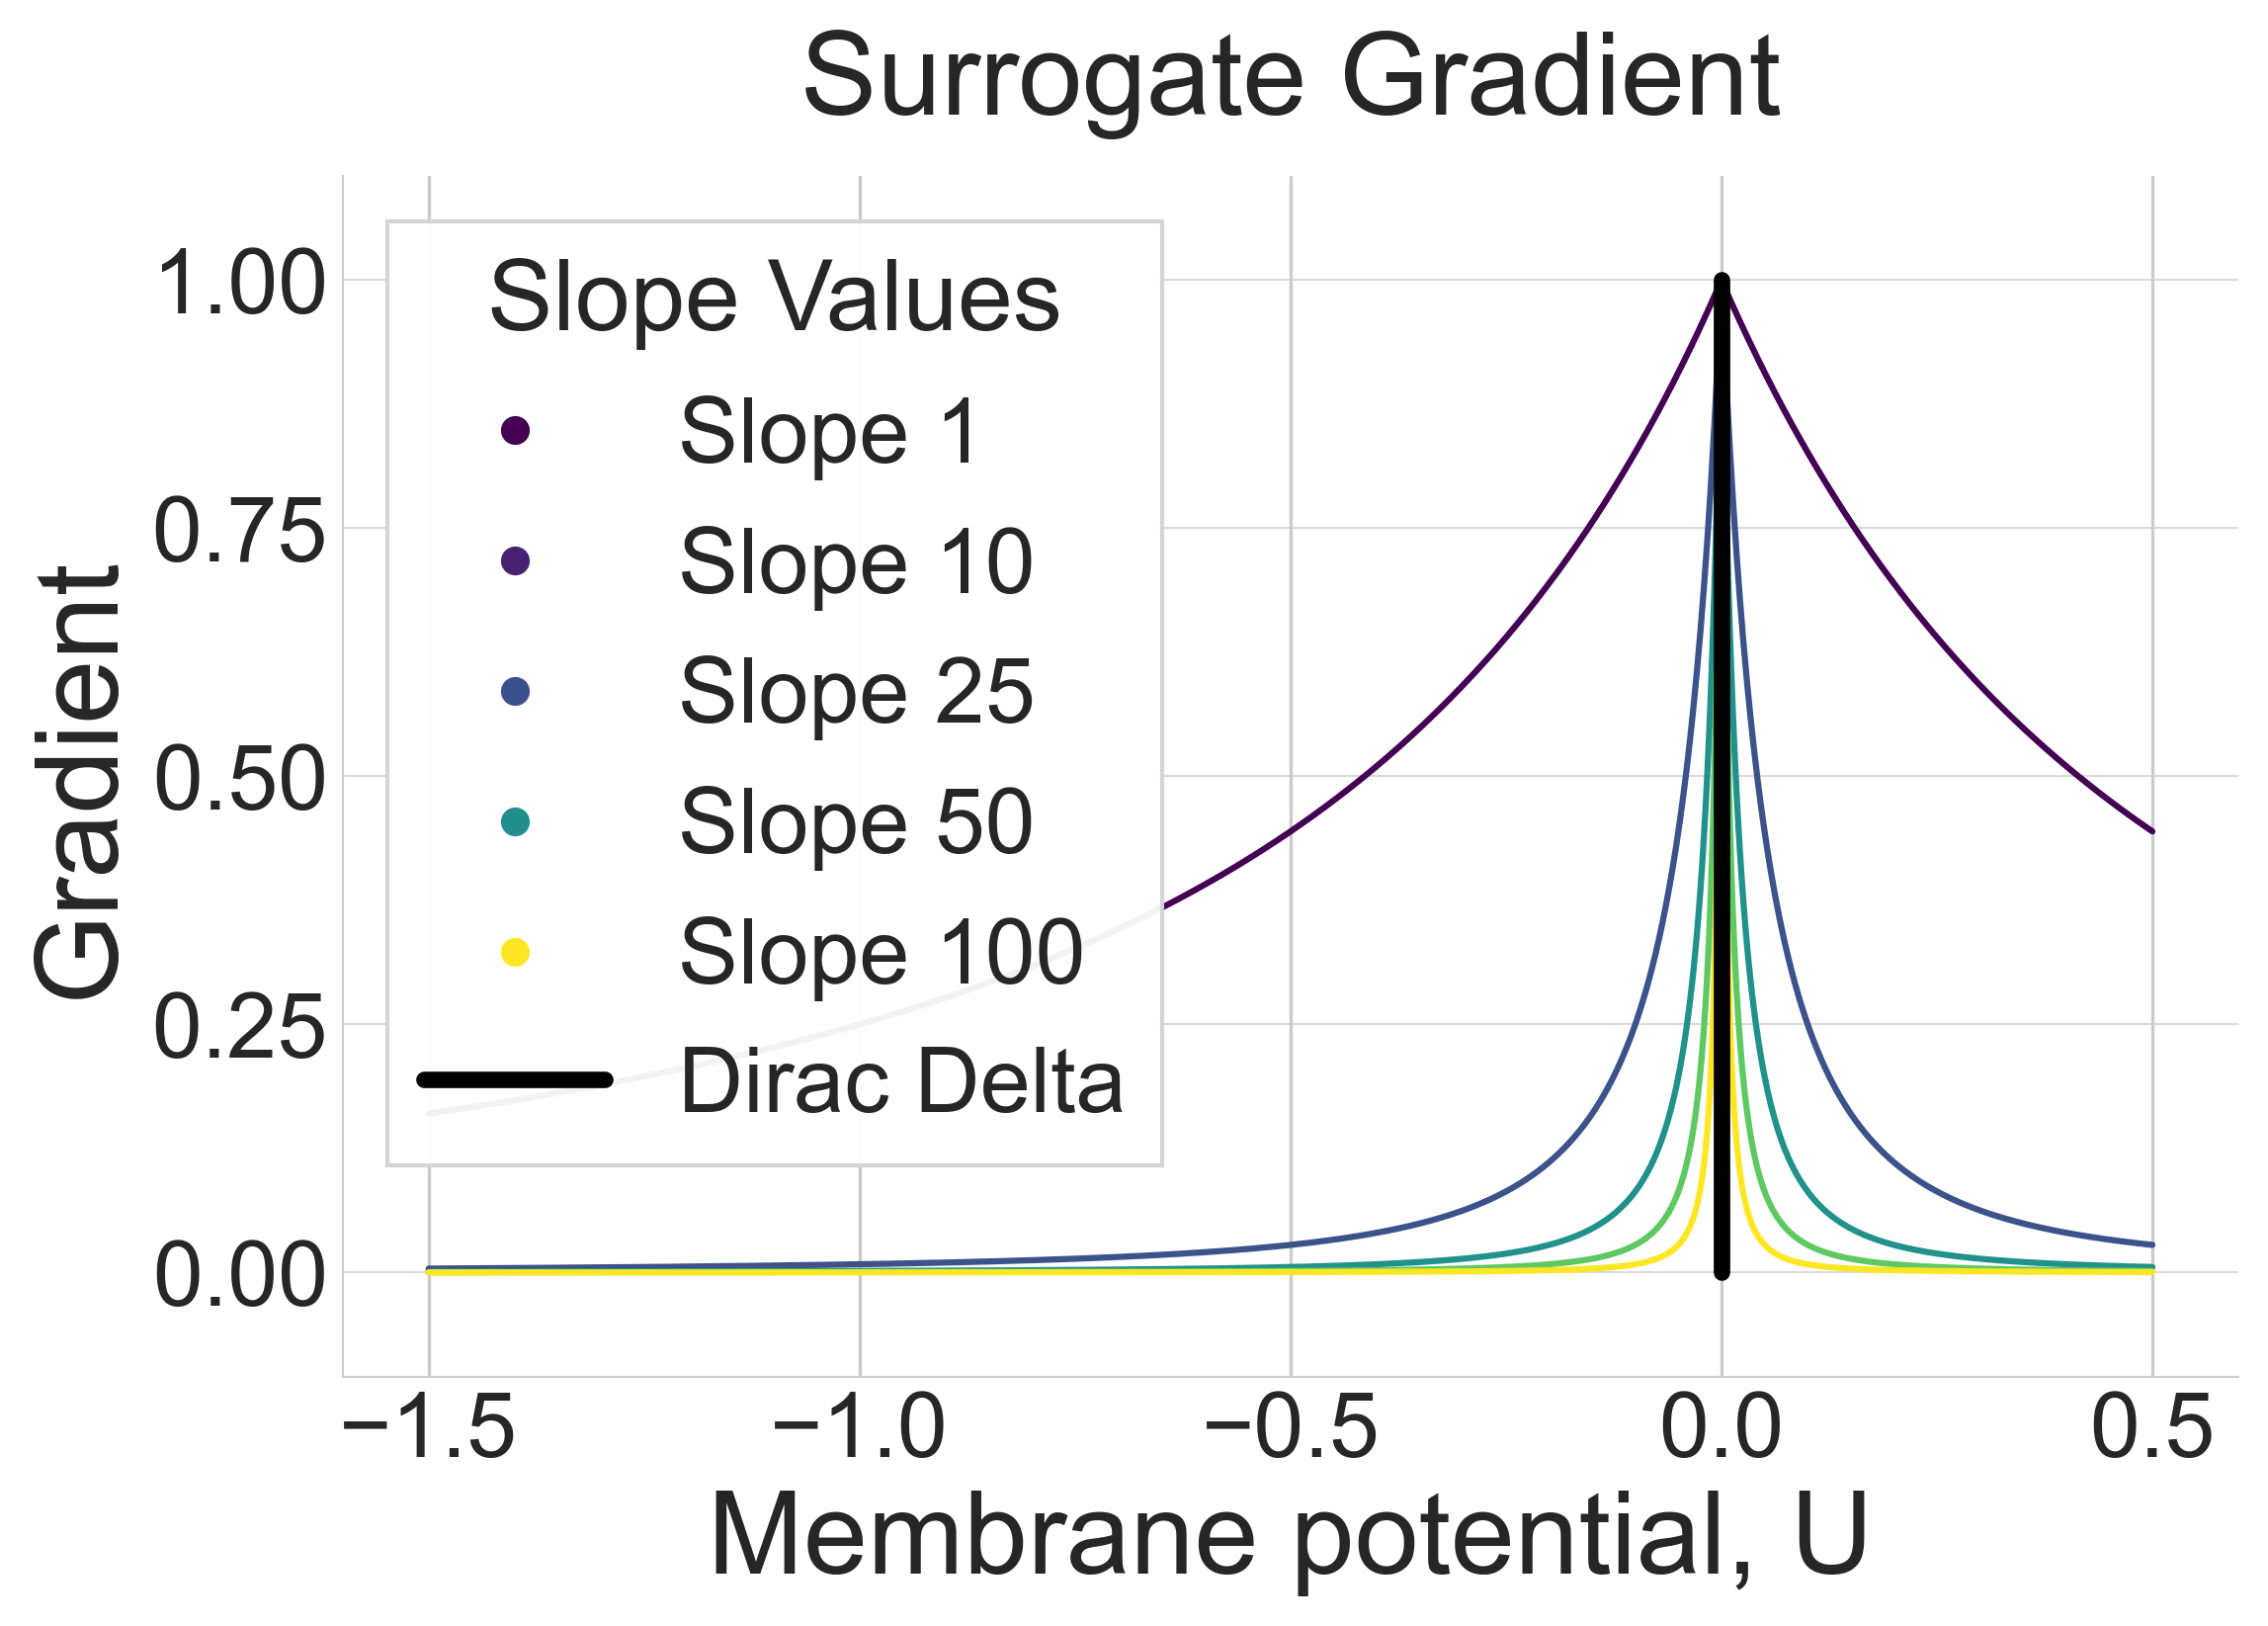
\includegraphics[height=3.6cm]{figures/neurips_surrogate_gradients.png}
        \caption{The slope of the surrogate gradient dictates the range of inputs for which a gradient exists.}
        \label{fig:surrslope}
    \end{subfigure}
    \hspace{0.02\textwidth}
    \begin{subfigure}[t]{0.31\textwidth}
        \centering
        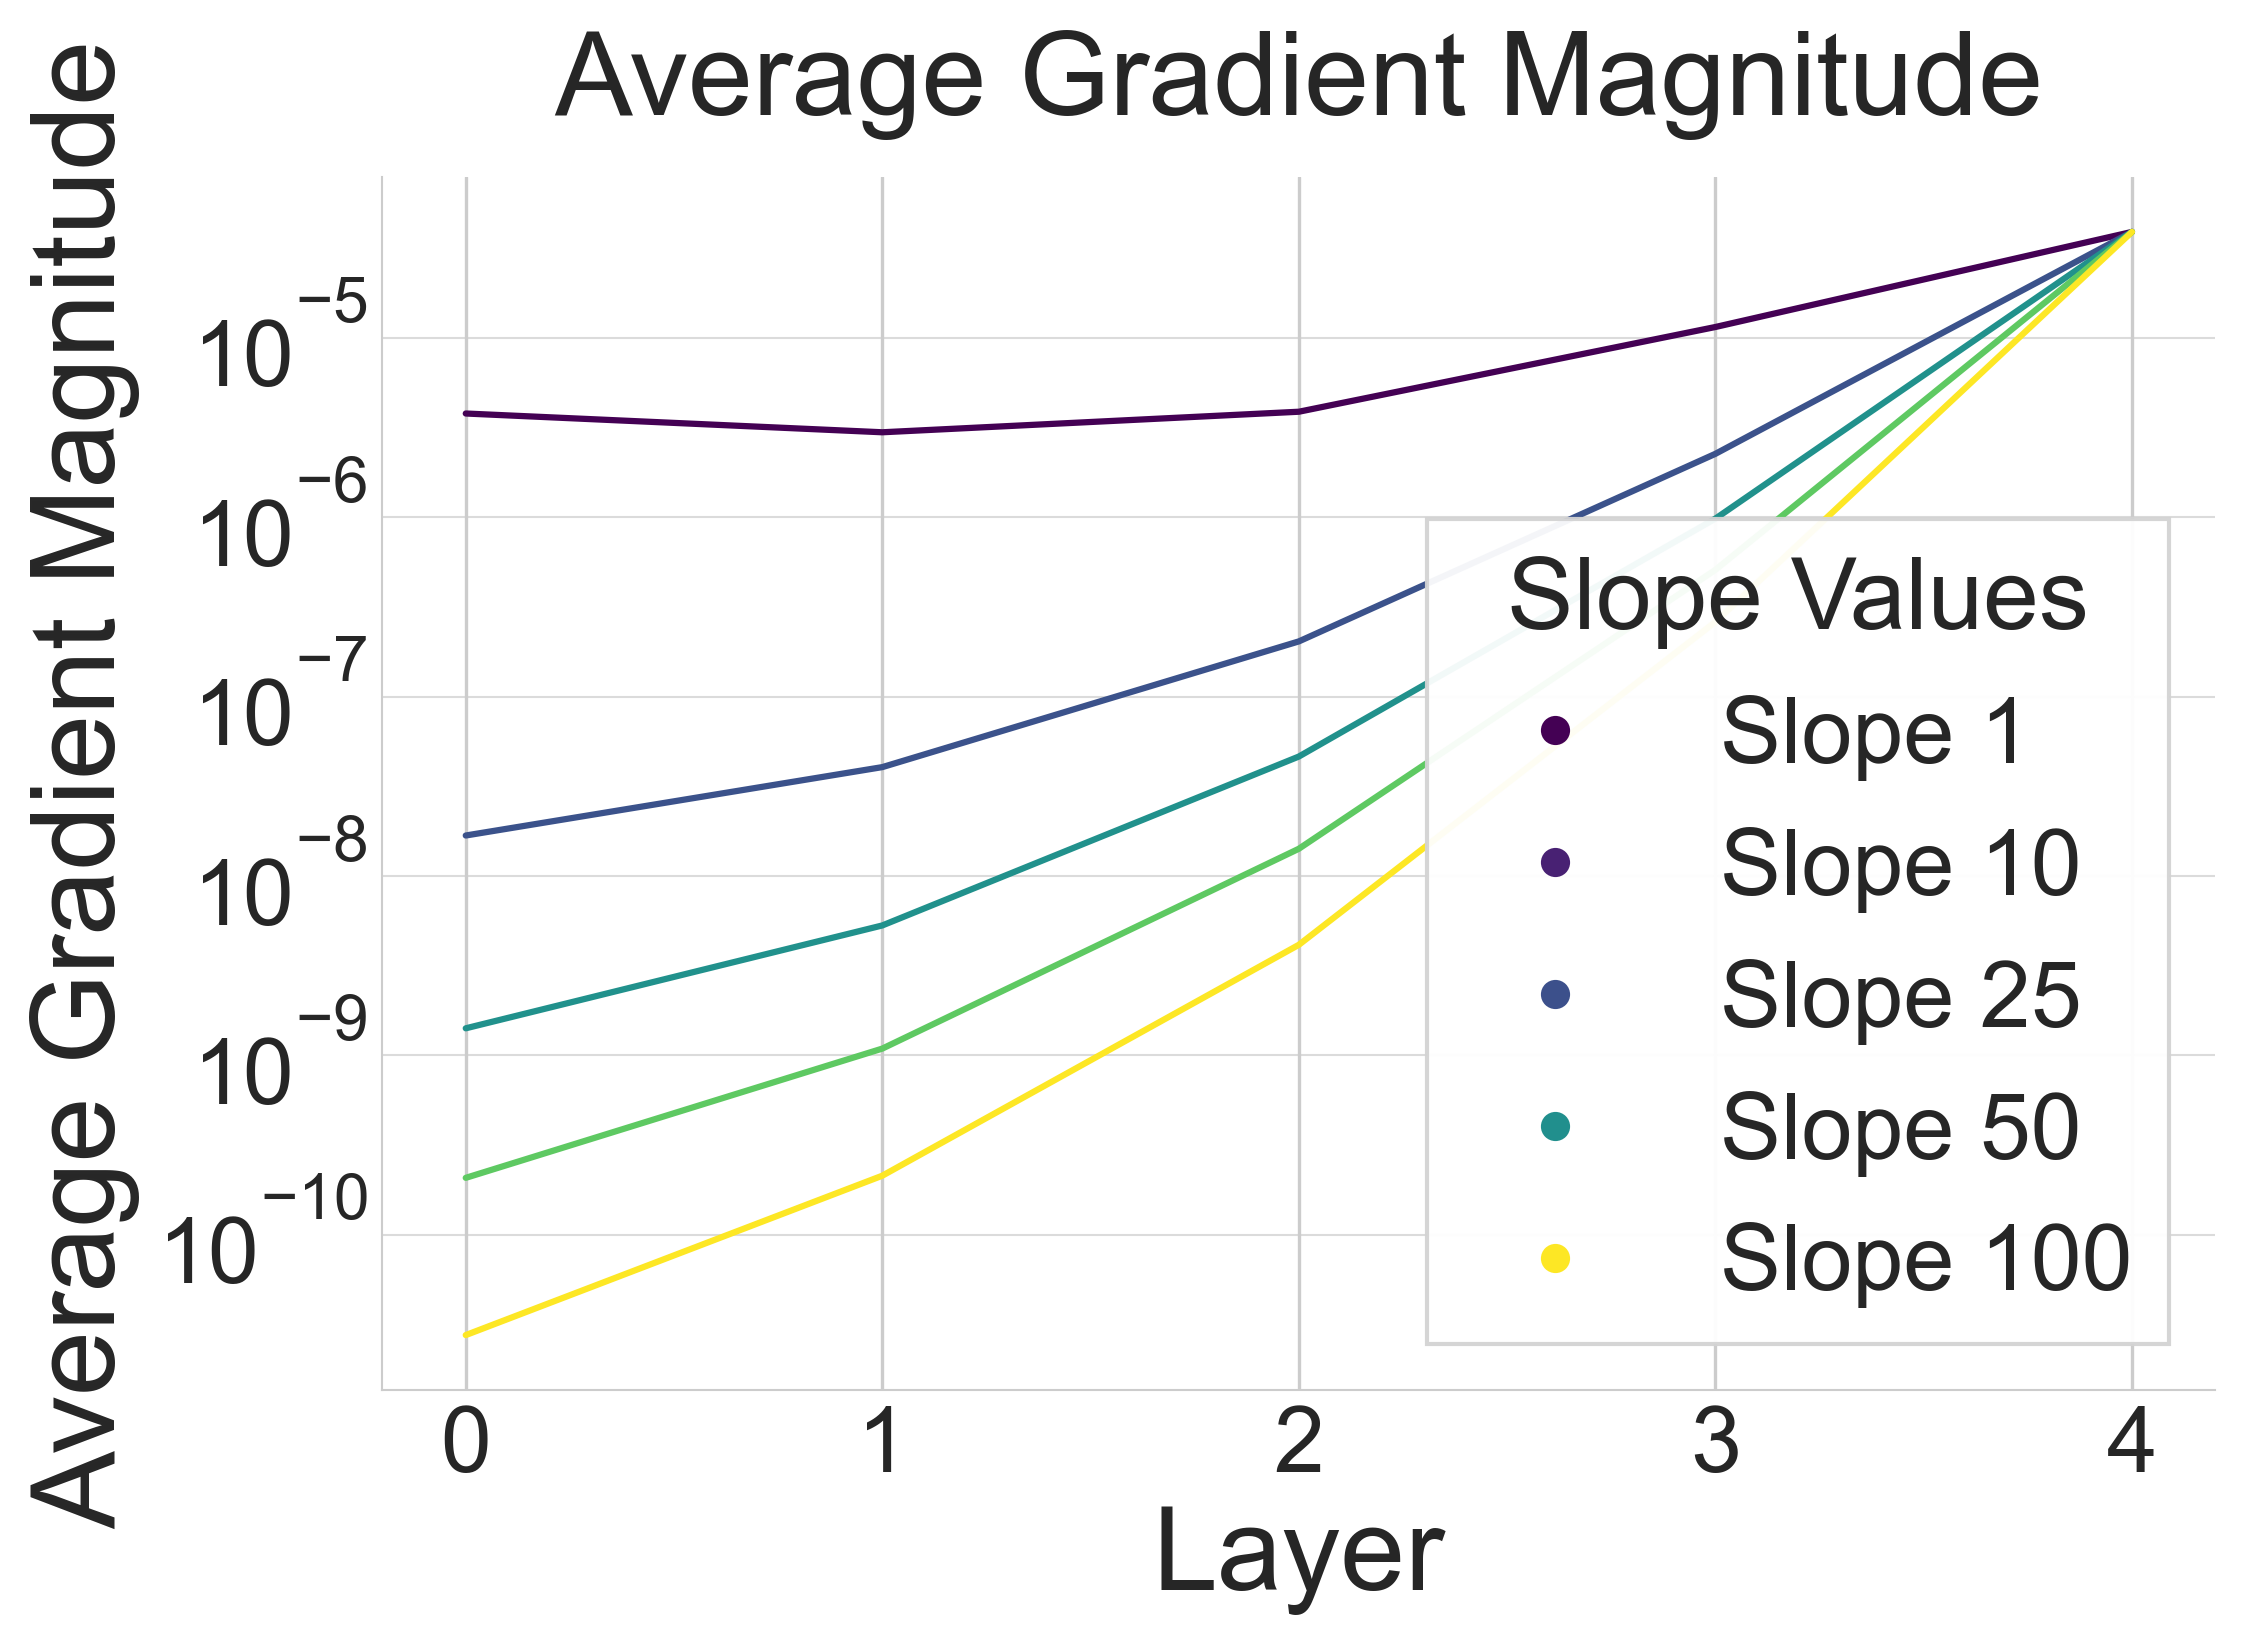
\includegraphics[height=3.6cm]{figures/neurips_avg_grad_magnitude.png}
        \caption{A more shallow slope carries the gradient deeper through the network, suffering less from vanishing gradients.}
        \label{fig:gradmagn}
    \end{subfigure}
    \hspace{0.02\textwidth}
    \begin{subfigure}[t]{0.31\textwidth}
        \centering
        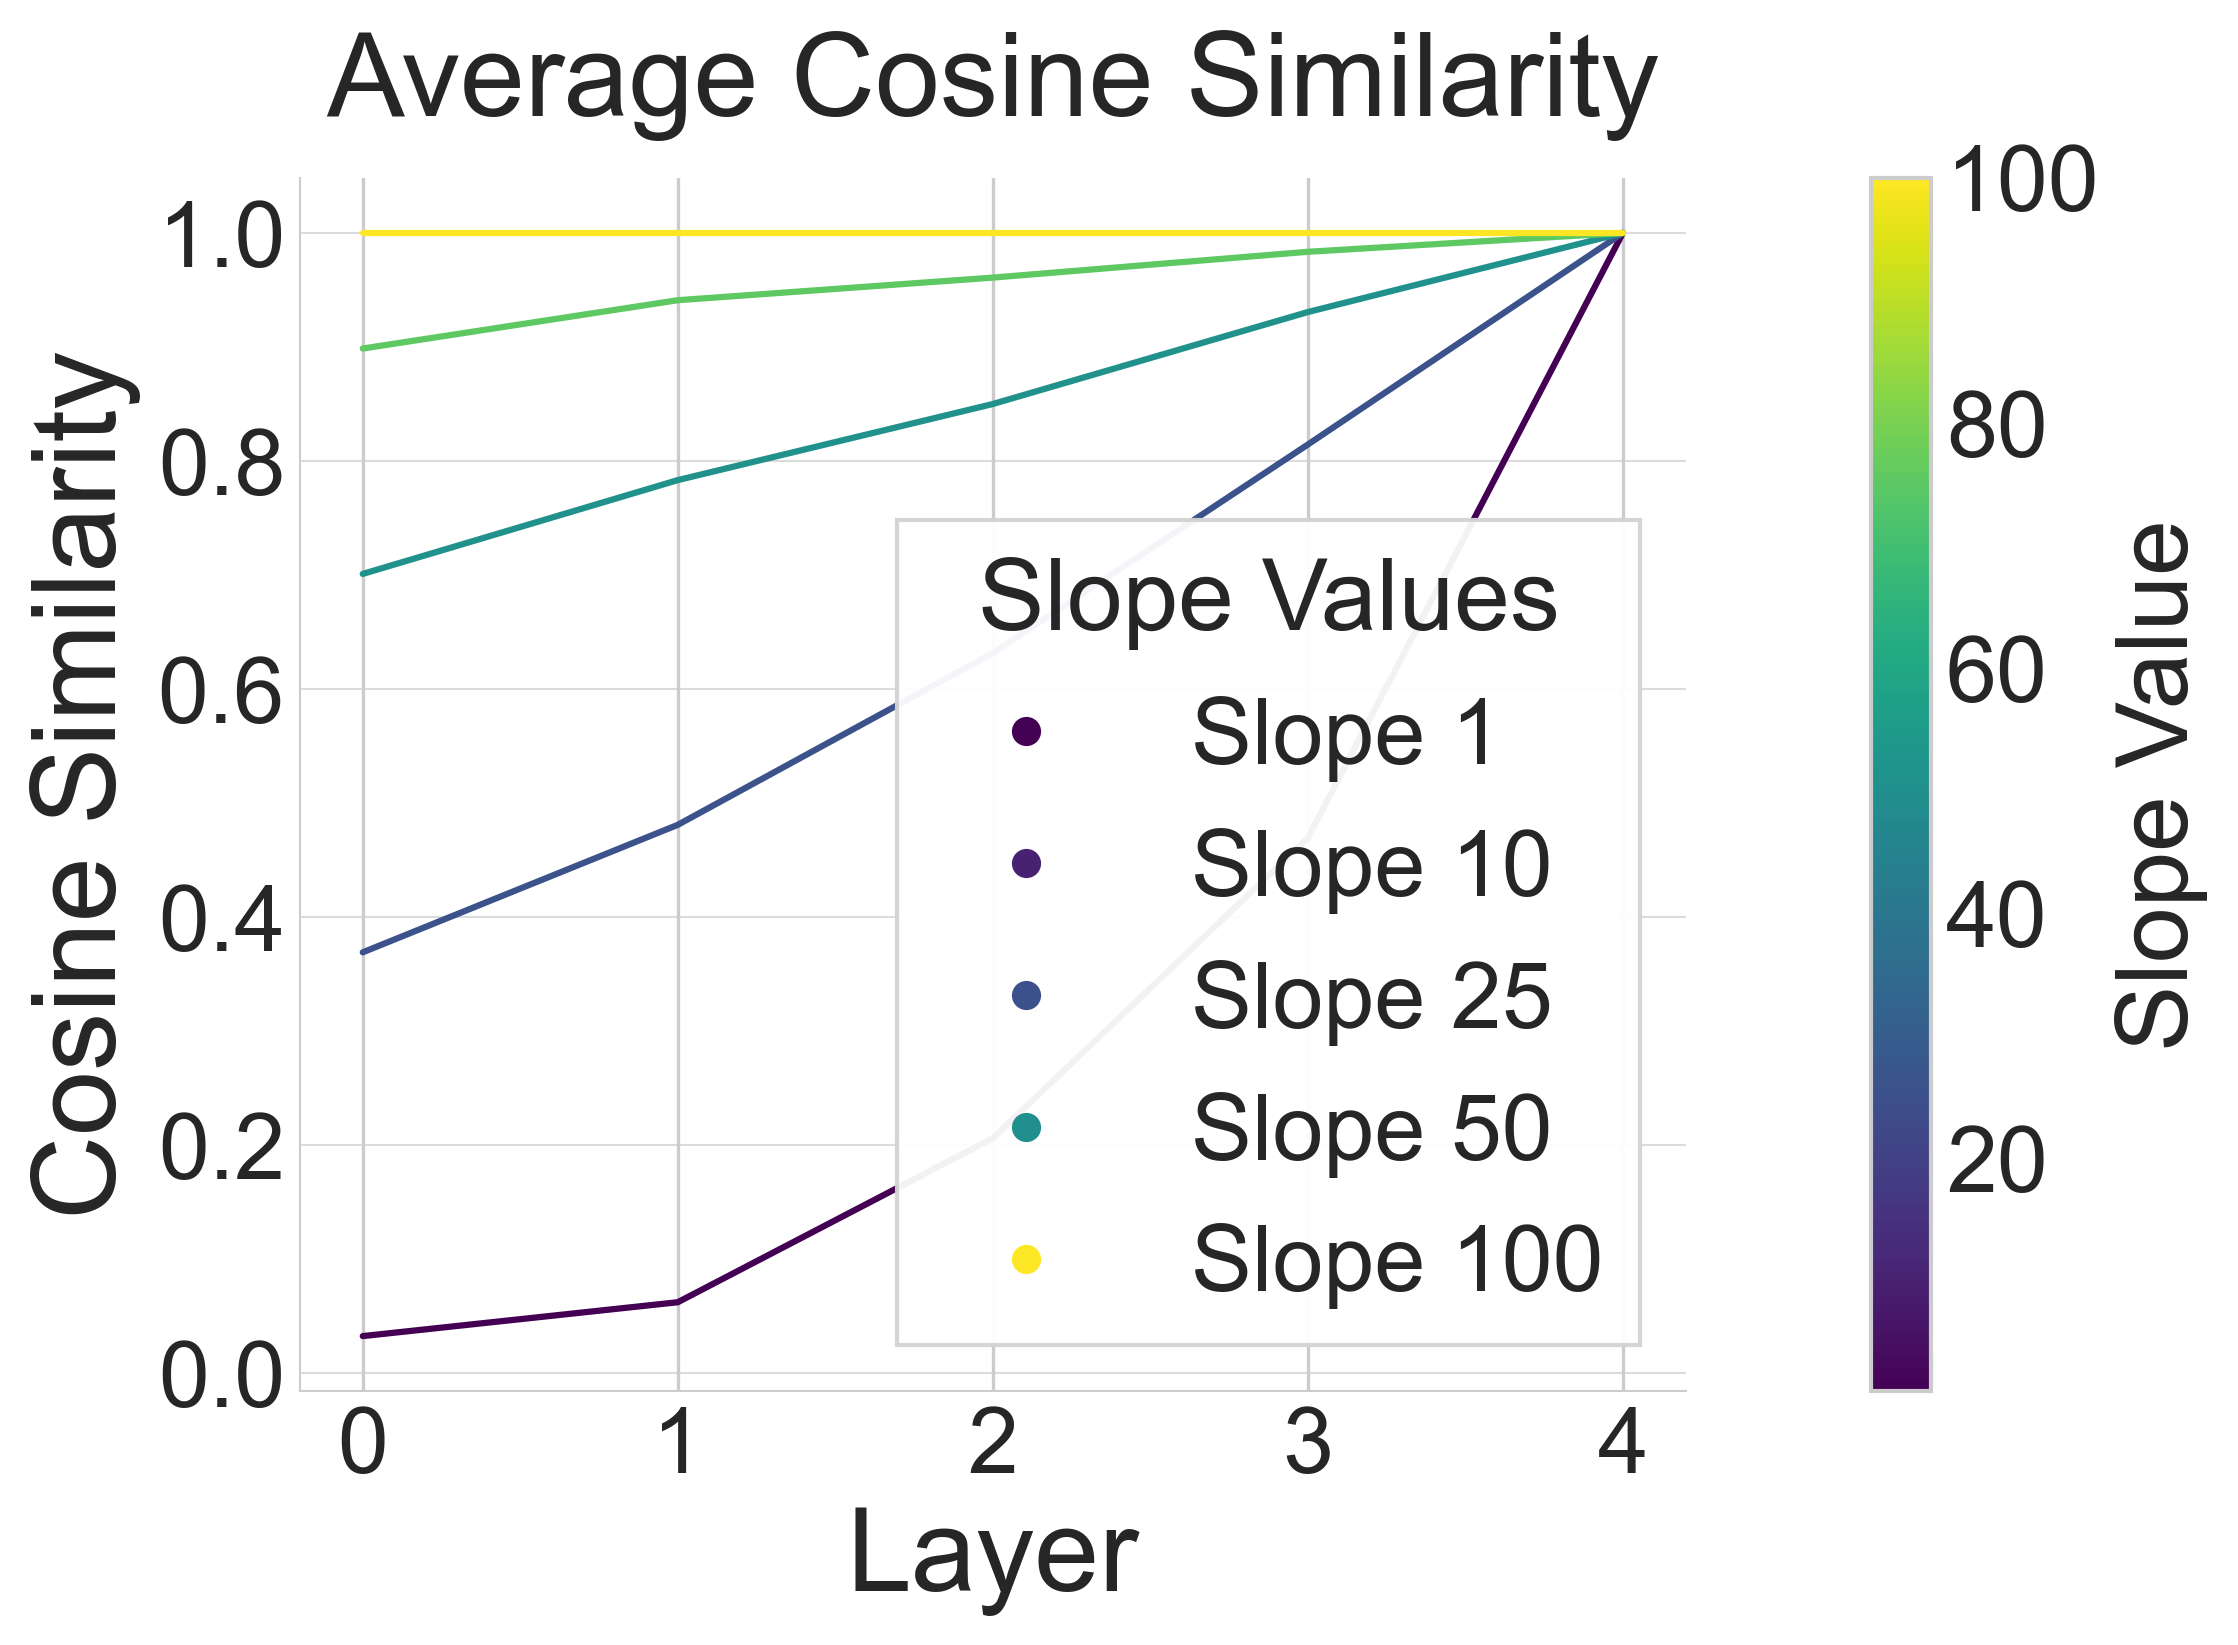
\includegraphics[height=3.6cm]{figures/neurips_cosine_similarity_line.png}
        \caption{A shallower slope introduces bias and variance, computed using the cosine similarity. }
        \label{fig:cossim}
    \end{subfigure}
    
    \caption{The effects of surrogate gradients on gradients in deep networks. The network has 4 hidden layers; layer 0 is the first hidden layer, and layer 4 is the output layer.}
    \label{fig:fullwidthfigure}
\end{figure*}
Training SNNs via backpropagation requires the use of surrogate gradients to approximate the derivative of the non-differentiable spike function. A critical hyperparameter in this process is the slope $k$ of the surrogate function, which determines the sensitivity of the gradient near the spiking threshold.

We adopt a fast sigmoid function and examine slope configurations ranging from shallow ($k = 1$) to steep ($k = 100$). As shown in \autoref{fig:surrslope}, steeper slopes closely resemble the Dirac delta function but restrict non-zero gradients to a narrow input range. In contrast, shallower slopes lead to a greater number of non-zero gradients and thus increases the total gradient magnitude, particularly in deeper layers (\autoref{fig:gradmagn}).

While the surrogate gradient's slope affects the quantity of weight updates per backward pass, it also introduces noise into the gradient computation~\cite{GygaxElucidating}. Since the true gradient for deeper network layers does not exist, we analyze the relationship between a steep surrogate gradient ($k=100$), which approximates the true gradient $\nabla W_i$, and shallow surrogate gradients, denoted as $\tilde{\nabla}W_i$, using cosine similarity:
\begin{equation}
\text{cosine similarity} = \frac{\mathbf{\nabla W}_i \cdot \mathbf{\tilde{\nabla}W_i}}{\|\mathbf{\nabla W}_i\| \|\mathbf{\tilde{\nabla}W_i}\|}
\end{equation}
\autoref{fig:cossim} shows that the cosine similarity for shallow slopes reduce to $0$, therefore, the weight updates in deeper networks become essentially random.

\subsection{Surrogate Gradients During Training}
We now analyze the effect of surrogate gradient slope choices across both fully supervised, behavioral cloning (BC), and fully online training algorithms,  TD3 \cite{fujimoto2018addressing}. To eliminate the effect of the warm-up during training for this analysis, we do the following. We stack a history of observations, process multiple forward passes per observation and reset the SNN in between subsequent actions, similar to previous RL implementations for SNNs. 

In supervised learning, final performance is largely unaffected by the surrogate slope setting, though training dynamics vary. Shallow slopes add noise, requiring more updates, while steep slopes yield small gradient magnitudes, also slowing progress. In online RL, however, we observed a pronounced preference for much shallower slopes, where the reduced cosine similarity between the true and surrogate gradients introduces noise that naturally enhances exploration, similar to parameter noise \cite{plappert2017parameter}. During training, we found that the shallow slope settings in RL introduced higher variability in final performance across runs. Poor intermediate updates can corrupt the replay buffer with low-quality experiences, hindering convergence. Shallower slopes heighten this risk, making training less stable.

Next to fixed slope settings, two scheduling methods for the surrogate gradient slope were compared. Firstly, interval scheduling gradually changes the slope from $1$ to $100$ at a fixed interval during training. Secondly, adaptive scheduling uses a weighted sum of the low-passed first order derivative of the reward score history and the low-passed reward score itself, see \autoref{eq:adaptive}. Note that the proportional term is largely responsible for not decreasing the slope when maximum performance is reached, and therefore destroying progress.
\begin{equation}\label{eq:adaptive}
    k_t = \frac{1}{10} \sum_{i=0}^{9} \left[0.5 r_{t-i} + 0.5 r'_{t-i}\right]
\end{equation}
Where $k_t$ is the slope at time $t$, $r_{t-i}$ is the reward score at time $t-i$ and $r'_{t-i}$ is the first order derivative of the reward score at time $t-i$.

We observe that scheduled slope settings firstly improve the training efficiency, greatly reducing the number of epochs to reach a reward of $100$. Secondly, final performance of the trained agents lie in the same regime as fixed slope experiments. When it is unsure what surrogate gradient is needed, scheduled approaches can eliminate the need for exhaustive hyperparameter sweeps accross different slope settings to identify the best performing ones. However, we find that an optimal slope exists which can outperform both interval and adaptive scheduling.

\begin{figure*}[h!]
    \centering
    \begin{subfigure}[b]{0.49\textwidth}
        \centering
        
\includegraphics[width=\textwidth]{figures/neurips_time_to_100_plot.png}
        \caption{The slope of the surrogate gradient dictates the range of inputs for which a gradient exists. The real gradient of the step function is the Dirac Delta.}
        \label{fig:surrslope}
    \end{subfigure}
    \hfill
    \begin{subfigure}[b]{0.49\textwidth}
        \centering
        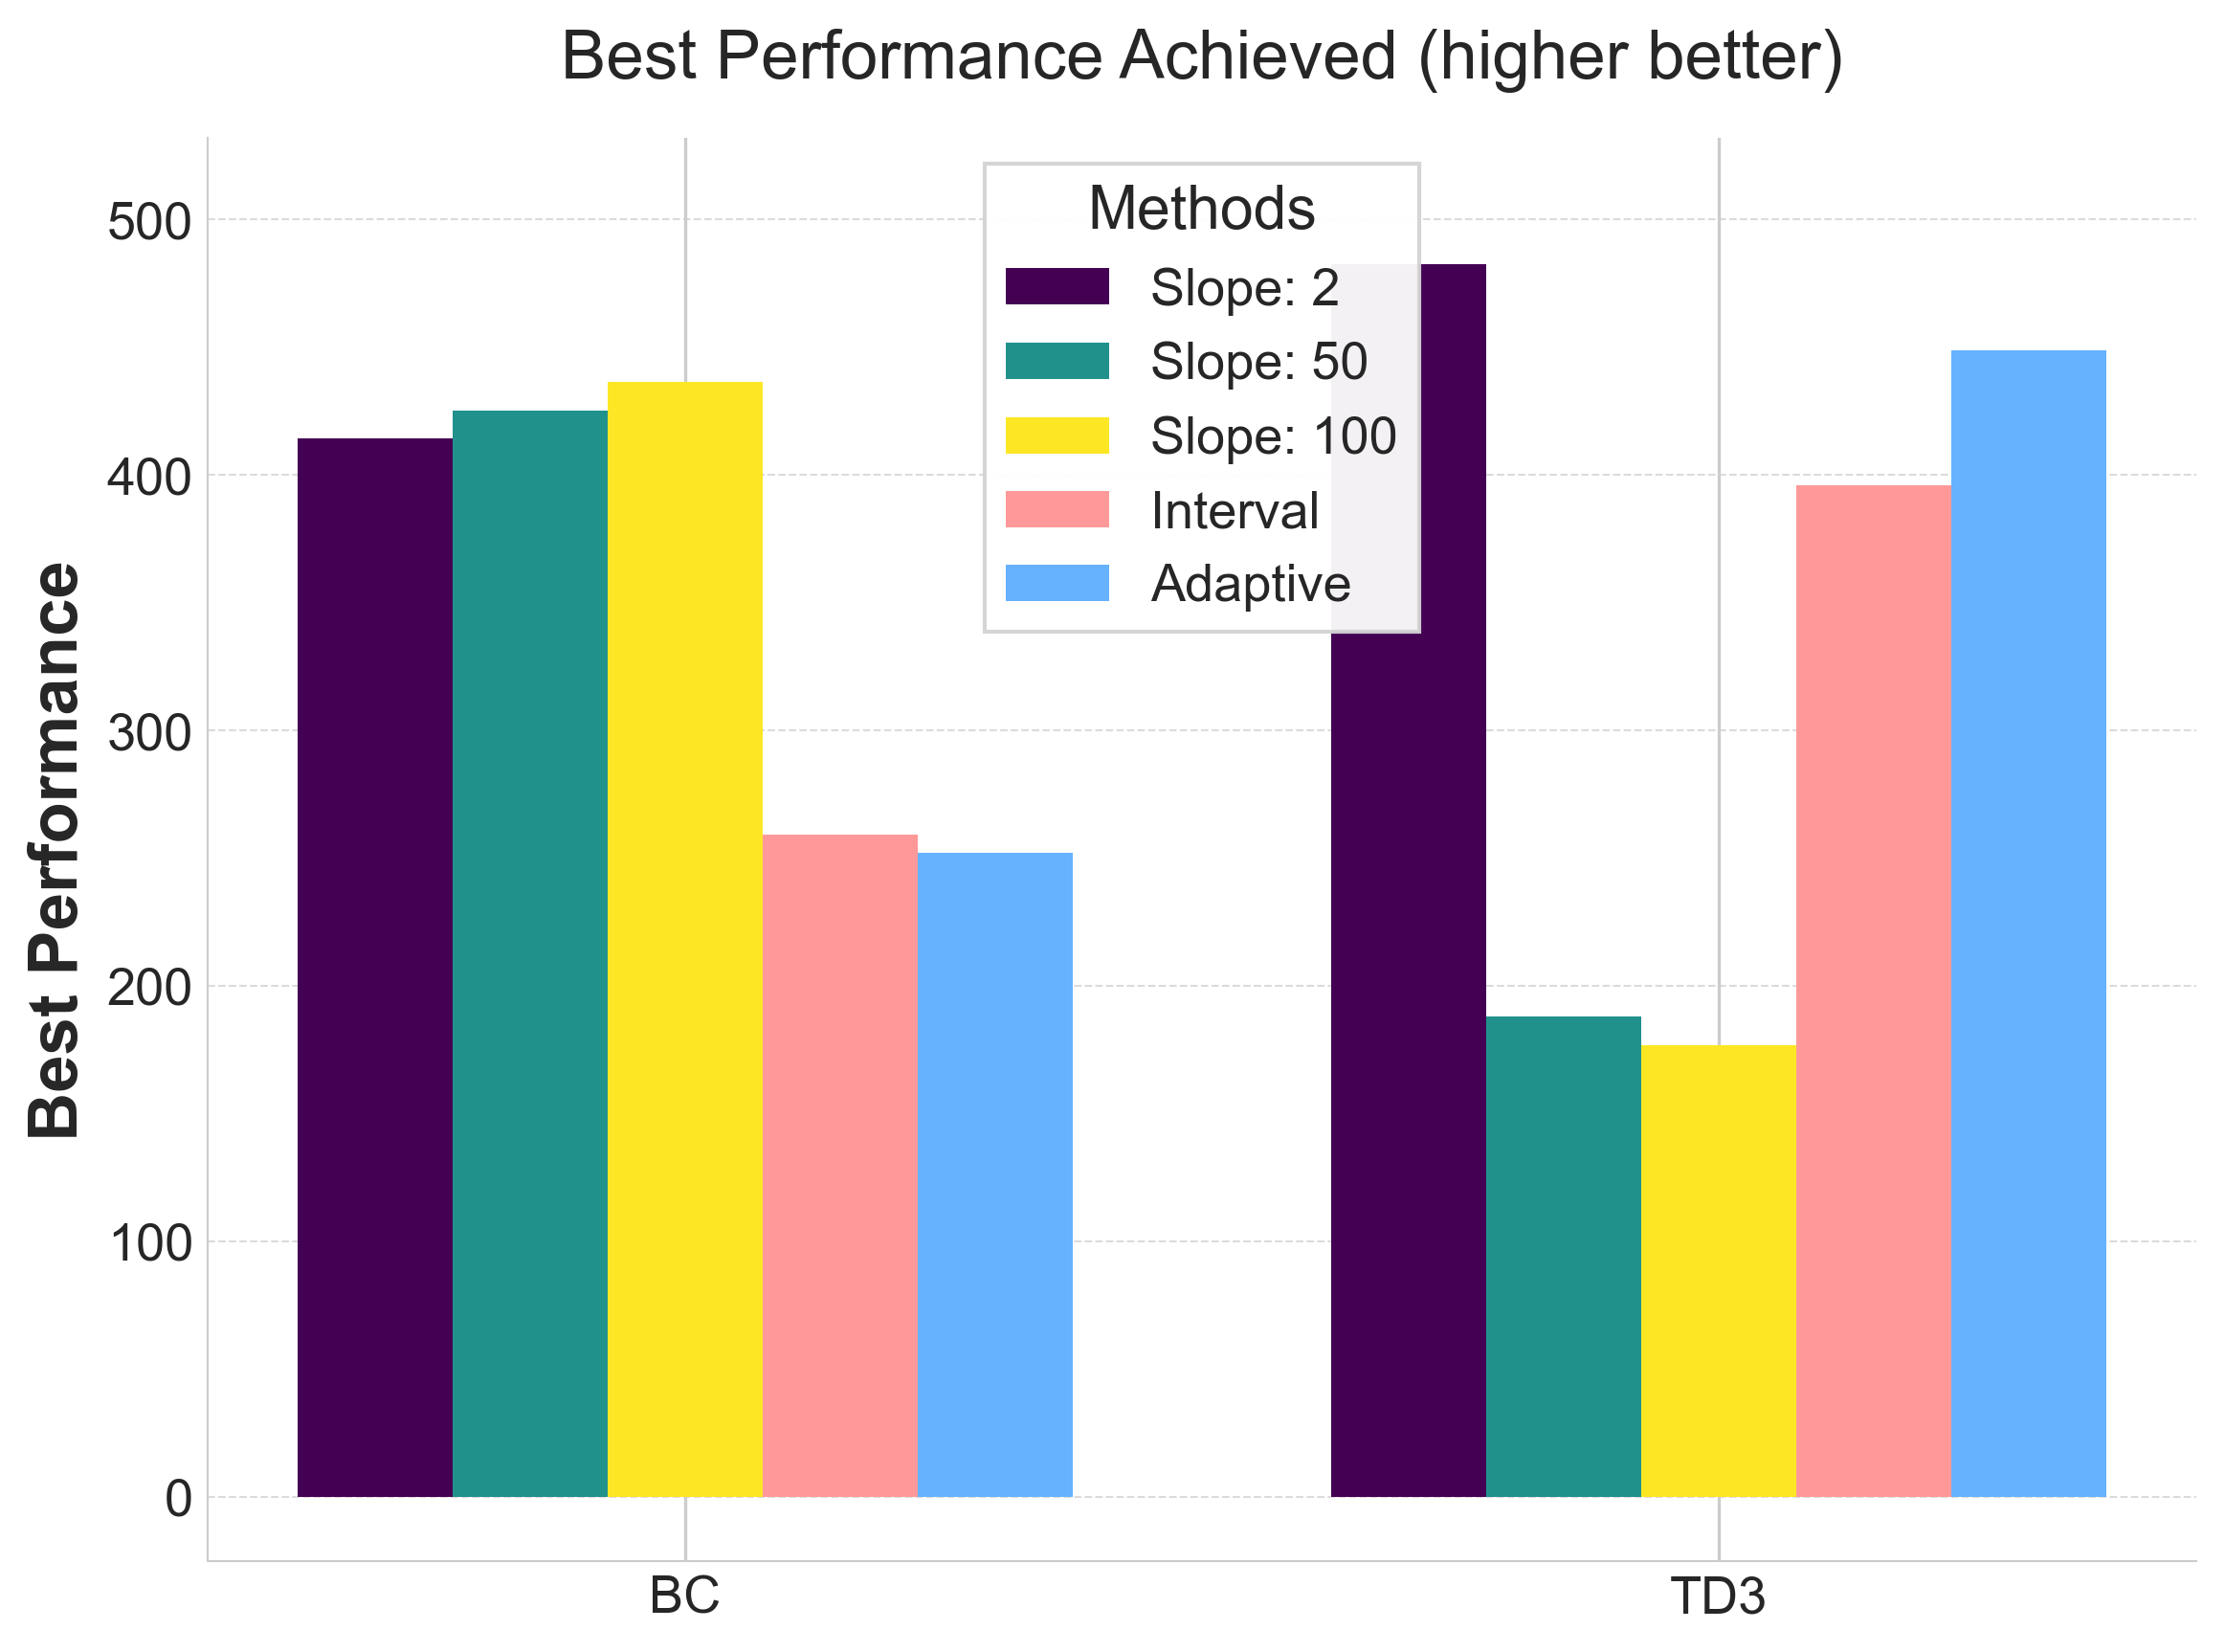
\includegraphics[width=\textwidth]{figures/neurips_best_performance_plot.png}
        \caption{A more shallow slope carries the gradient deeper through the network, therefore suffering less from the vanishing gradient problem. }
        \label{fig:gradmagn}
    \end{subfigure}
    \caption{The effects of surrogate gradients on the gradients computed for deep networks. The network has 4 hidden layers, where layer 0 relates to the first hidden layer, up until layer 4 which is the output layer. All results are the average of 5 different seeds.}
    \label{fig:fullwidthfigure}
\end{figure*}

\subsection{Training on Sequences}
To fully leverage the temporal processing capabilities of SNNs in reinforcement learning, we extend training from single transitions to full sequences (\autoref{seq_snn}) and introduce a reward curriculum that gradually increases penalties on position, velocity, and action magnitude to encourage stable, robust behavior. The curriculum updates the penalties related to the aforementioned states at an interval of 10 epochs. All experiments use an adaptive slope scheduler for surrogate gradient slope adjustment. We compare BC, TD3BC, TD3, and TD3BC+JSRL. BC and TD3BC are offline RL algorithms trained on dataset sequences, gathered with the guiding policy used in our TD3BC+JSRL setup, while TD3 and TD3BC+JSRL are online algorithms sampling sequences from the environment. Unlike TD3, which starts from scratch, TD3BC+JSRL benefits from a privileged guiding policy during the first $n$ steps of rollouts. All approaches are evaluated under the reward curriculum and trained on an Apple MacBook Pro M4Pro, with $24GB$ RAM.
\begin{figure*}[h!]
    \centering
    \begin{subfigure}[b]{0.49\textwidth}
        \centering
        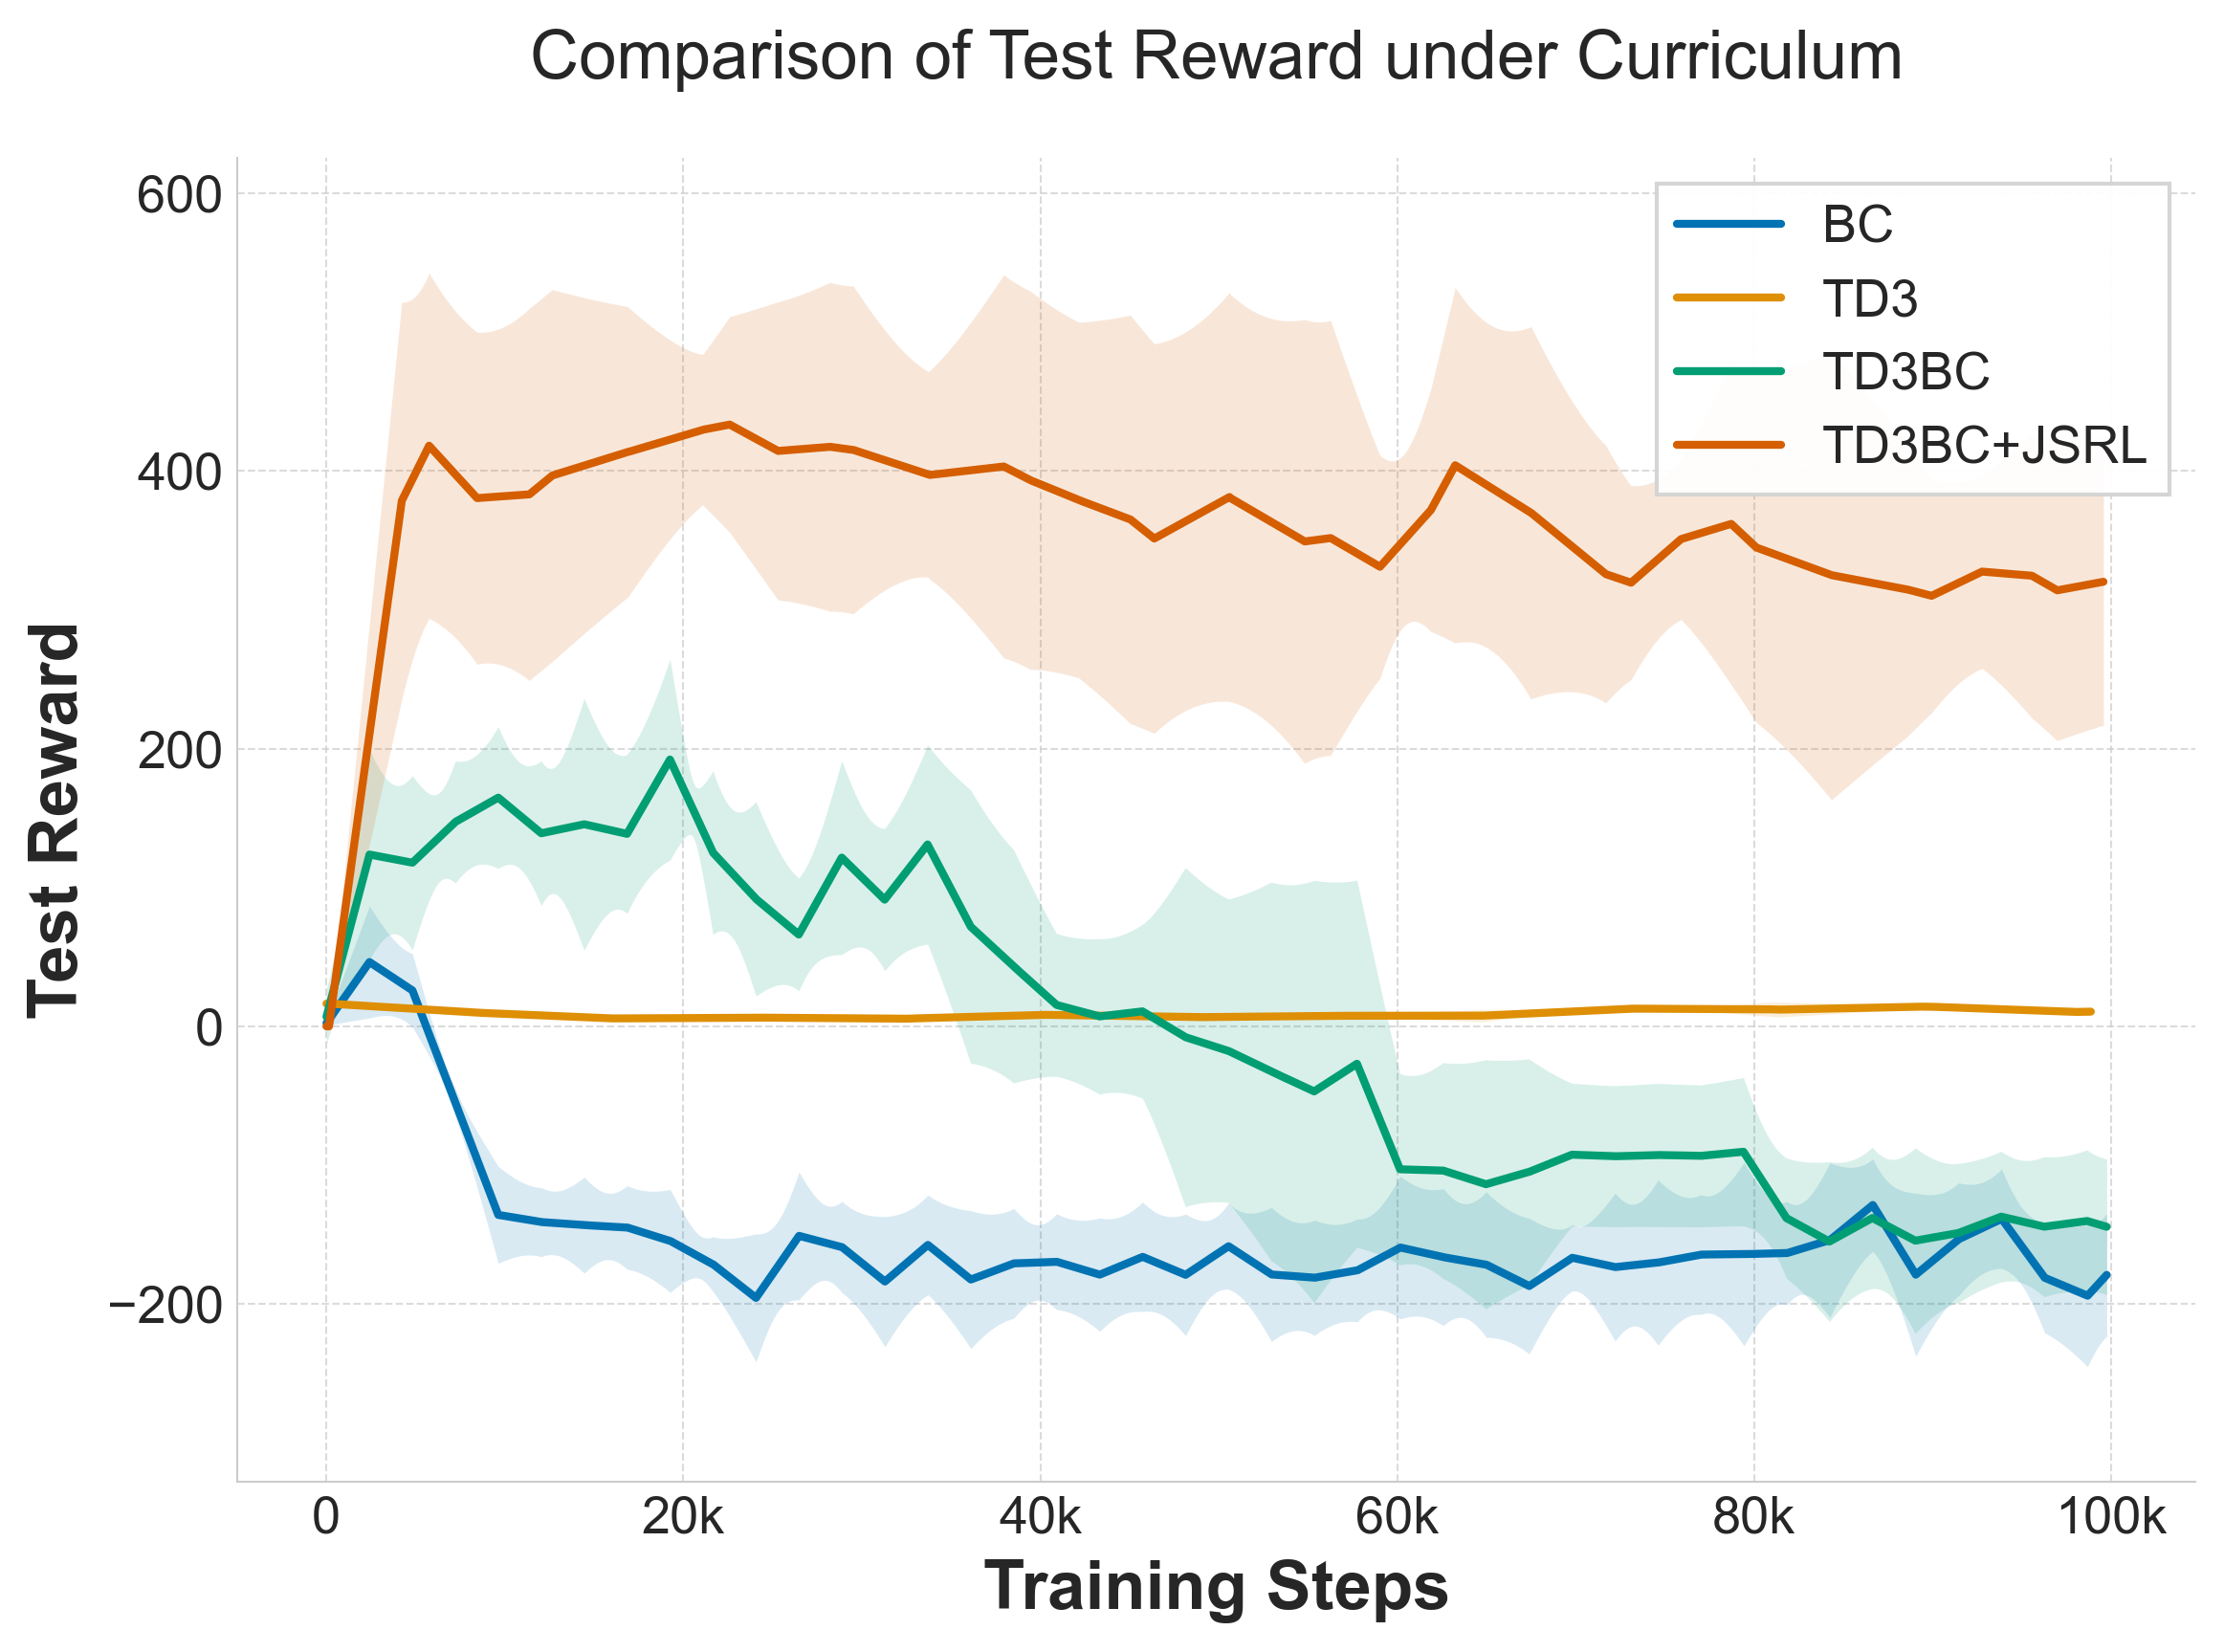
\includegraphics[width=\textwidth]{figures/neurips_comparison_plot_reward.png}
        \caption{Offline methods (BC and TD3BC) struggle as the reward function adapts, failing to generalize beyond the initial dataset.}
        \label{fig:rews_training_methods}
    \end{subfigure}
    \hfill
    \begin{subfigure}[b]{0.49\textwidth}
        \centering
        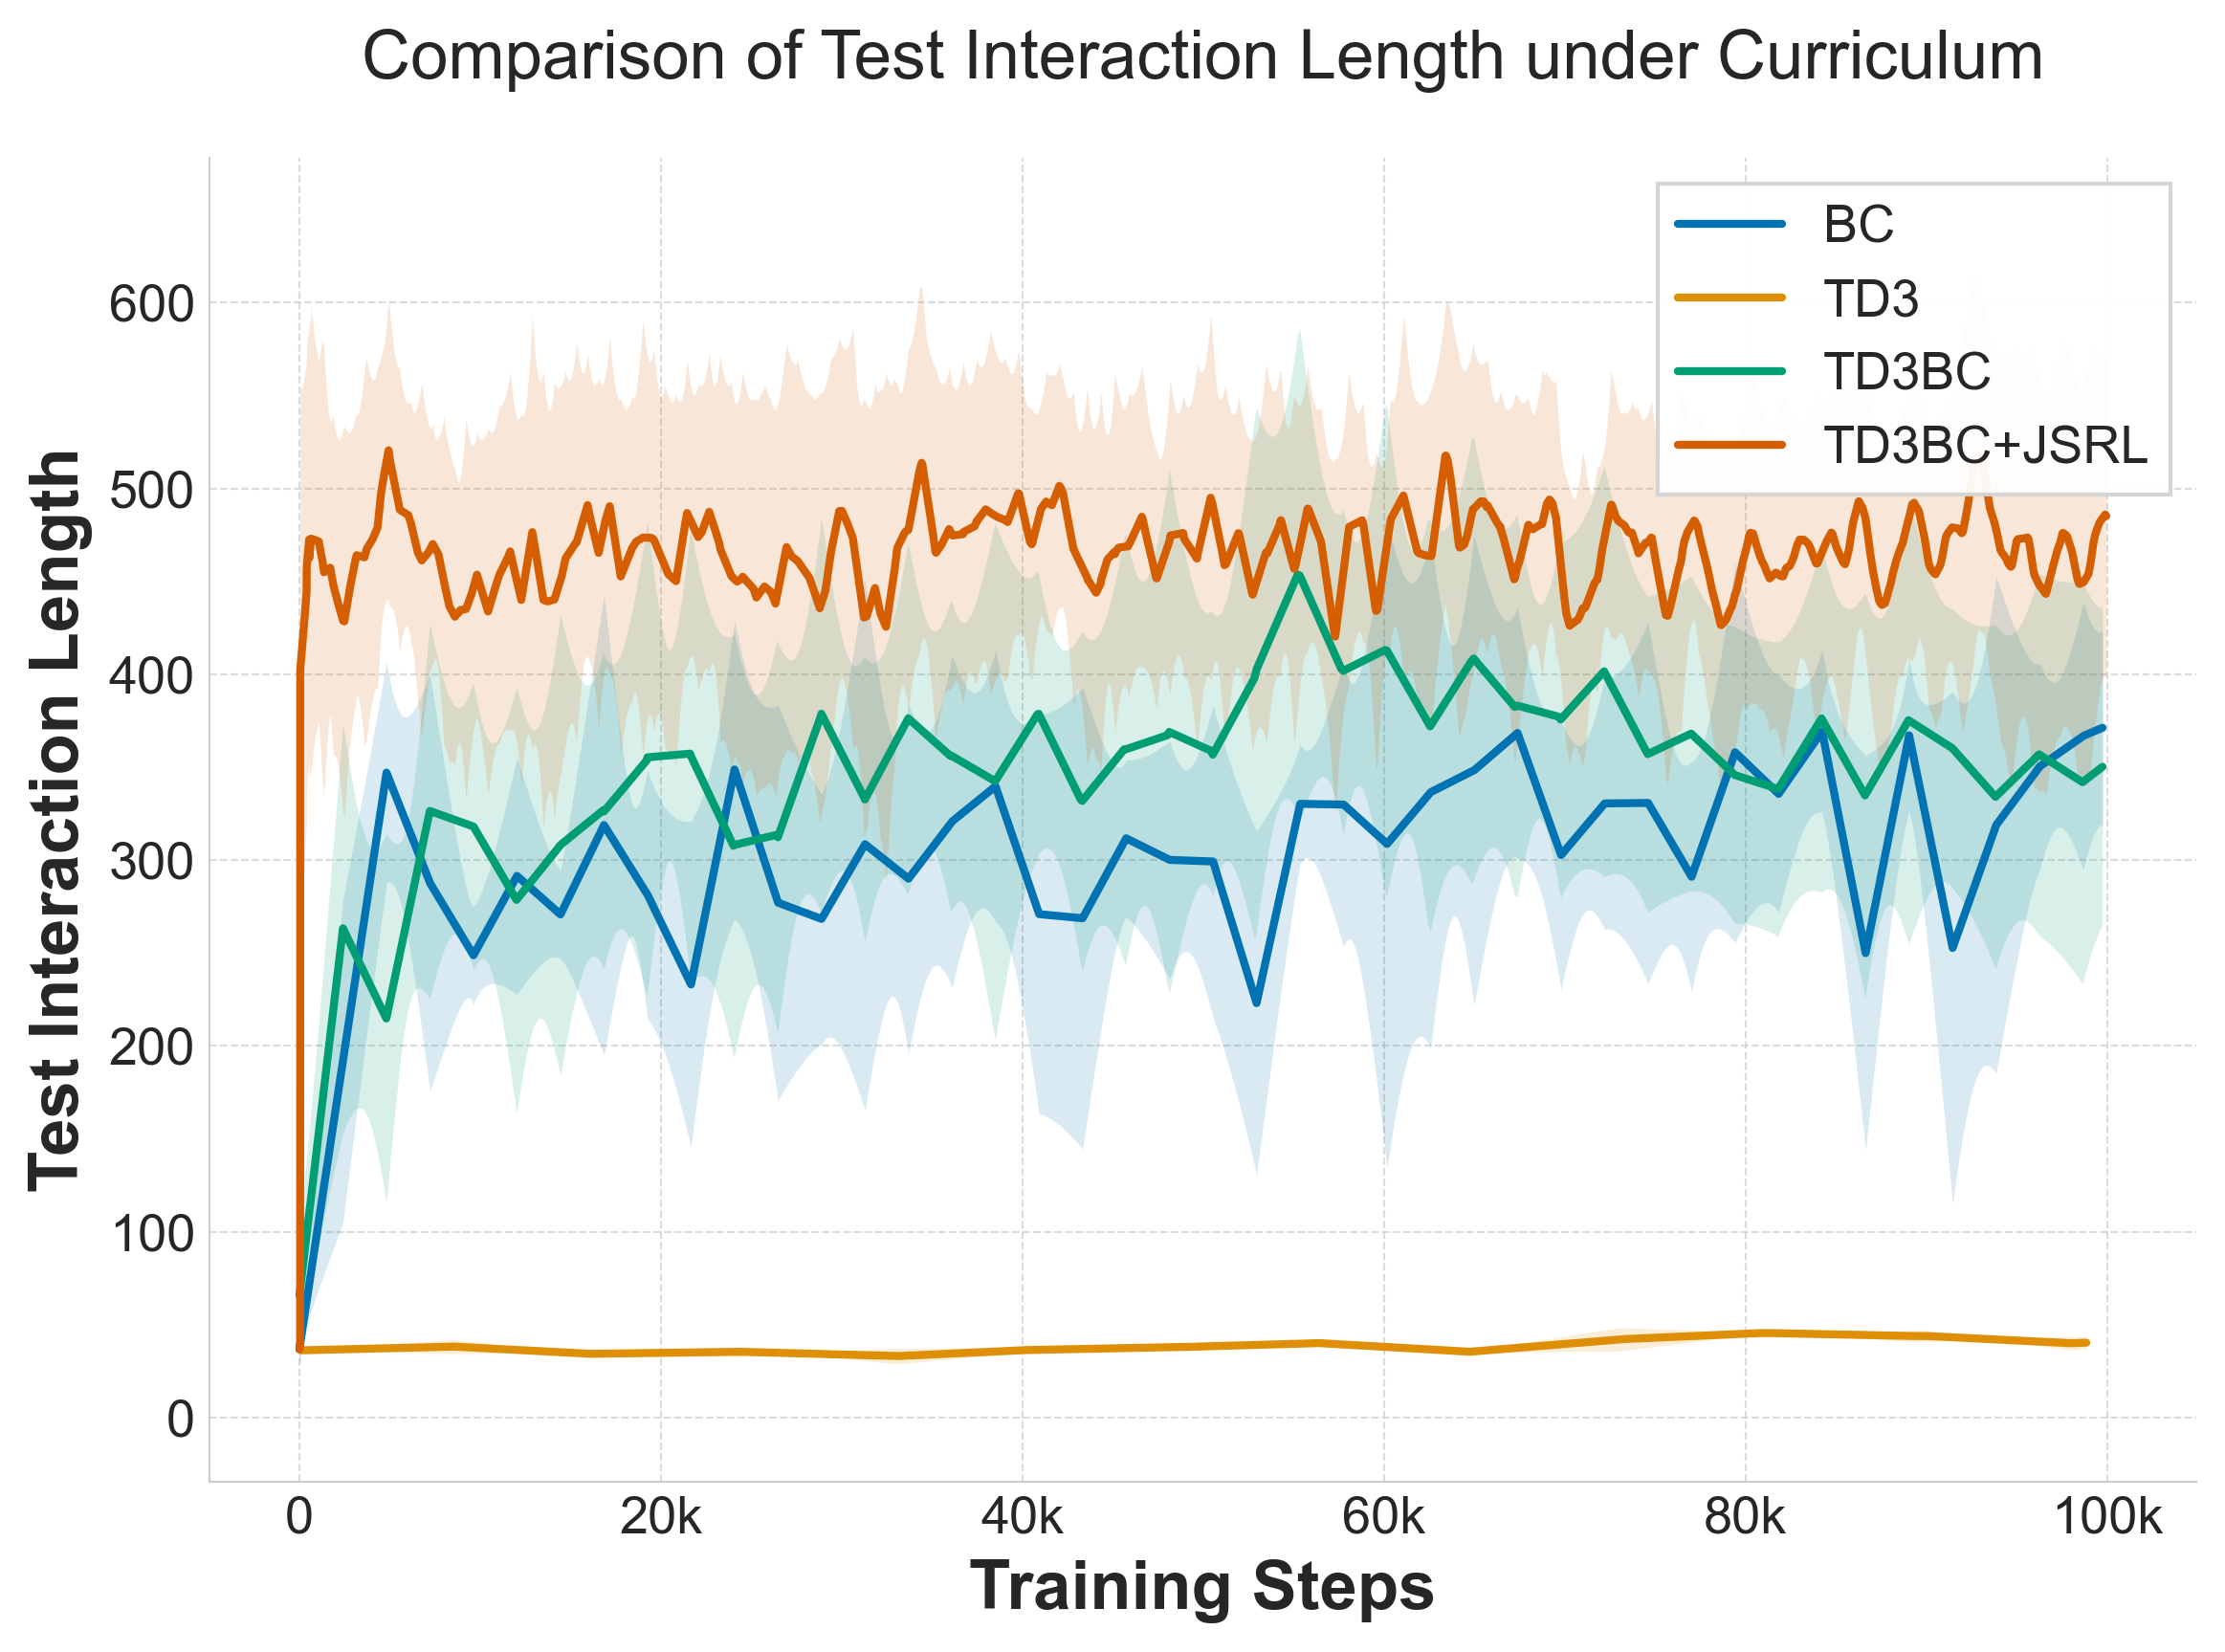
\includegraphics[width=\textwidth]{figures/neurips_comparison_plot_lens.png}
        \caption{While all methods, except TD3, eventually learn to fly, TD3-trained policies frequently terminate early due to unstable exploration, whereas TD3BC+JSRL achieves longer and more stable flight trajectories.
}
        \label{fig:lens_training_methods}
    \end{subfigure}
    \caption{Comparison of training approaches under a reward curriculum. All experiments were ran with 5 different seeds.}
    \label{fig:fullwidthfigure}
\end{figure*}

BC suffers from the unseen curriculum, as shown in \autoref{fig:rews_training_methods}. Next, TD3BC \cite{FujimotoMinimal} initially shows the ability to leverage reward information to surpass the baseline BC training performance. However, as the reward function diverges from the dataset, the performance of the controller greatly drops, to the performance of the baseline BC controller. While TD3 has access to evolving interactions, it struggles to gather meaningful sequences early in training, often resulting in premature episode terminations, as seen on \autoref{fig:lens_training_methods}, failing to bridge the warm-up period. Our proposed TD3BC+JSLR approach, which incorporates new rollouts guided by a privileged policy, demonstrates robust learning even under a challenging curriculum. The inclusion of online rollouts enables the model to adapt to the evolving reward landscape, leading to substantial performance improvements.

The hyperparameters, curriculum and training details used for the experiment are part of the supplementary materials.

\subsection{Bridging the Reality Gap}
We quantitatively evaluated the computational efficiency of our sequential SNN approach using NeuroBench \cite{yik2023neurobench}. Results show that temporally-trained SNNs match ANN performance while exhibiting distinct computational traits. Despite a higher memory footprint, SNNs benefit from activation sparsity and primarily use energy-efficient accumulates (ACs) instead of energy-hungry multiply-accumulates (MACs), making them well-suited for neuromorphic deployment.

\begin{table}[h]
\centering
\renewcommand{\arraystretch}{1.5}
\begin{tabular}{c|c|c|c|c|c|c|c} \thickhline
Model & \makecell{Reward\\} & \makecell{Footprint\\(kb)} & \makecell{Activation\\Sparsity} & \makecell{SynOps\\Dense} & \makecell{SynOps\\Eff\_MACs} & \makecell{SynOps\\Eff\_ACs} &\makecell{Requires\\History}\\ \hline
$ANN$ & $447$ & $55.3$ & $0.0$ & $13.7\times 10^{3}$ & $13.7\times 10^{3}$ & $0.0$ &True\\
$SNN$ & $446$ & $158.3$ & $0.79$ & $37.9 \times 10^{3}$ & $4.6\times 10^{3}$ & $12.2\times 10^{3}$ & False\\ \thickhline
\end{tabular}
\caption{NeuroBench performance comparison between ANN (64-64 architecture) and temporally-trained SNN (256-128 architecture) using TD3BC+JSRL.}
\label{tab:NeuroBenchResults}
\end{table}
When deployed on the Crazyflie, the SNN controller exhibits oscillatory behavior, likely due to limited output resolution and lack of explicit action history. However, the SNN is still able to execute complex maneuvers like circles (see \autoref{fig:realCrazyFlie}), eight figures and squares. ANN controllers, benefiting from full action history, show smoother control.

To improve stability, future work could incorporate angular velocity penalties, throttle deviation outputs, longer training, or increased control frequency, as prior work has shown smoother SNN control at higher rates \cite{Eschmann2023,stroobants2024neuromorphic}.
\begin{figure}[b]
    \centering
    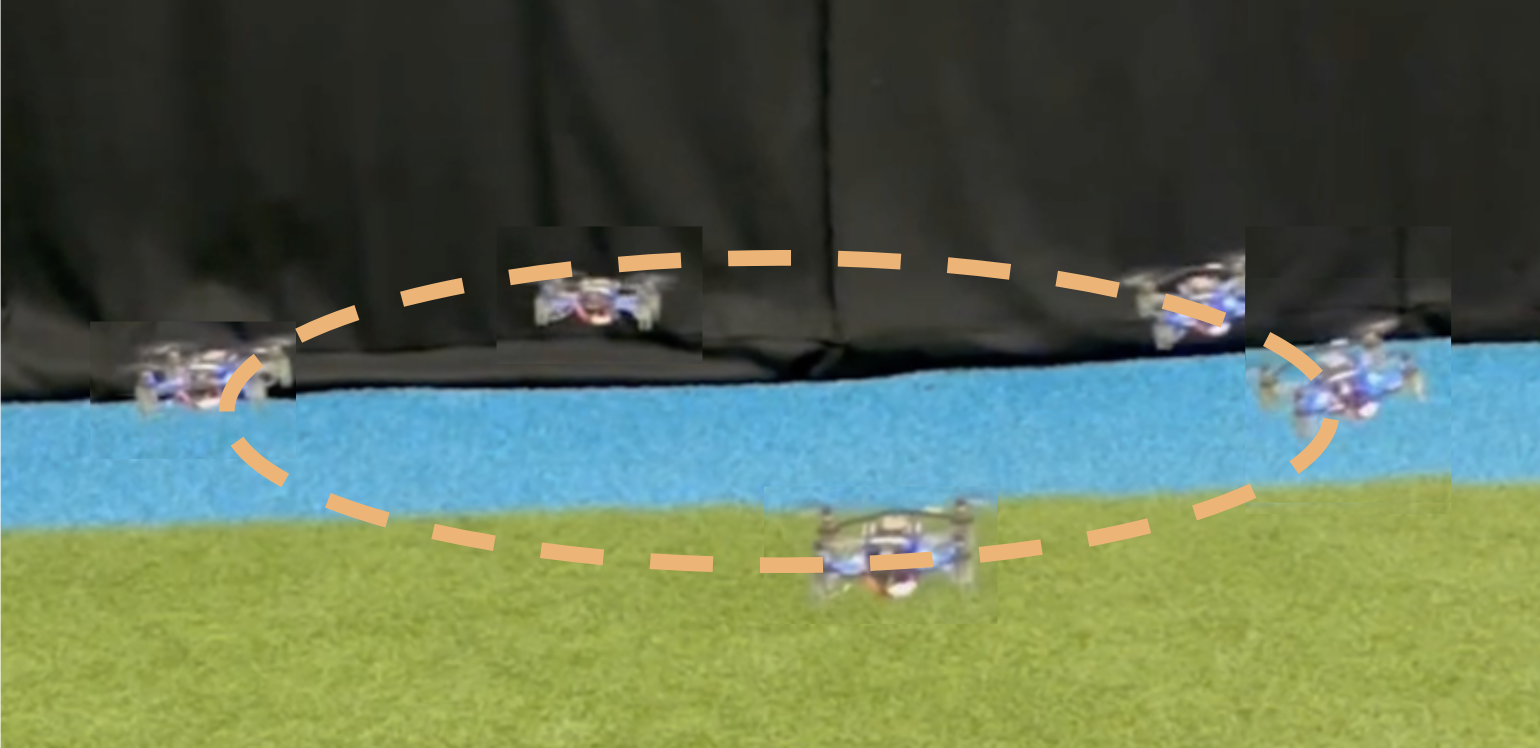
\includegraphics[width=0.47\textwidth]{figures/CrazyFlieFlight.png}
    \caption{When deployed on the CrazyFlie, the spiking actor displays oscillatory behavior, but can successfully fly maneuvers such as circles.}
    \label{fig:realCrazyFlie}
\end{figure}
We deployed the trained SNNs on Crazyflie variants with standard and modified motor-propeller setups. Compared to ANN controllers from Eschmann et al. \cite{Eschmann2023}, SNNs achieved lower position error under ideal conditions but had reduced reliability. Notably, while ANNs without action history failed to control the drone, our SNN leveraged temporal dynamics to maintain control, albeit with occasional crashes.

\begin{table}[h!]
\centering
\renewcommand{\arraystretch}{1.5}
\begin{tabular}{c|c|c|c|c} \thickhline
& \makecell{ANN\\action history \cite{Eschmann2023}} & \makecell{ANN\\no action history \cite{Eschmann2023}} & SNN & \makecell{SNN\\altered drone} \\ \hline
\makecell{Position Error [m]} & 0.1 & 0.25 & 0.04 & 0.14 \\\hline
\makecell{Trajectory Error [m]} & 0.21 & $\infty$ & 0.24 & 0.20 \\ \thickhline
\end{tabular}
    \caption{Comparison of neural network models for position control and trajectory tracking tasks. The models include an ANN with full observation and action history, an ANN without action history, an SNN trained with TD3BC+JSRL without action history, and the same SNN deployed on a drone with modified motors and propellers. The mean position error of the deployed SNNs is benchmarked against the best-performing ANN policy \cite{Eschmann2023}. Position error is measured as the average xy-plane error (in meters), and trajectory tracking error is evaluated as the average error across figure-eight and square-following tasks.}

    \label{tab:comparison}
\end{table}
